%! Author = charon
%! Date = 1/2/23

\section{Einführung}\label{sec:einfuhrung}
% kurz erklären und einführen wieso die begriffe wichtig sind und hinleiten zum kernthema log4j
%%erklären wieso manche sachen nur briefly behandeln
Diese Arbeit beschäftigt sich mit dem \gls{cve}-2021-44228, auch bekannt als Log4Shell. Bei dieser Schwachstelle handelt es sich
um einen Zero-Day-Exploit. Unter einem Zero-Day-Exploit versteht man "[die] Ausnutzung einer Schwachstelle, die nur dem Entdecker bekannt ist [...]."\footcite{bsizeroday}
Die Schwachstelle wurde am 09. Dezember 2021 entdeckt. Betroffen hierbei war die oft eingesetzte Bibliothek log4j (Version 2).\footcite{lunasec} In den
folgenden drei Kapiteln werden zuerst grundlegende Begriffe eingeführt, die zum Verständnis im weiteren Verlauf der Arbeit wichtig sind.
Zudem werden in dieser Arbeit einige Technologien, wie beispielsweise die tatsächliche Implementierung des Loggers oder Serialisierung der Objekte in der
\gls{jvm}, grob umrissen.
%! Author = johannes
%! Date = 03.01.23

\subsection{Log4j}\label{subsec:log4j}
\begin{wrapfigure}{r}{0.33\textwidth}
    \begin{center}
        
\includegraphics[width=0.3\textwidth]{images/log4j}
    \end{center}
    \caption{Log4j Logo}
\end{wrapfigure}
Log4j 2 ist eine von Apache entwickelte open-source Logging Library für Java.
Heutzutage als Standard-Library für Logging in Java bezeichnet, entstand Log4j 2 2012 aus einem kompletten rewrite der Log4j Library.
Log4j 2 ist komplett in Java geschrieben und bietet als großen Vorteil gegenüber dem Vorgänger auch Support für Plugins an.
Bis Version 2.12.1(06.08.2019) hat Log4j Java 7 vorausgesetzt, seit Version 2.13.0(11.12.2019)\footfullcite{log4jChange} wird Java 8 Version 2.4 verwendet.
Aufgrund des Standard-Logger Status von Log4j, wurde die Library in viele weitere Projekte aufgenommen.
So verwenden unter anderem Minecraft Java Edition, \gls{aws}, Cloudflare und Steam Log4j 2 in ihren Systemen.

%! Author = johannes
%! Date = 03.01.23

\subsection{JNDI}\label{subsec:jndi}
\begin{wrapfigure}{r}{0.5\textwidth}
    \begin{center}
        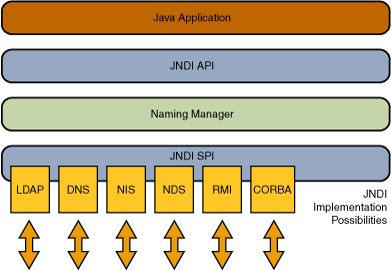
\includegraphics[width=0.48\textwidth]{images/jndiarch}
    \end{center}
    \source{\href{https://docs.oracle.com/javase/tutorial/jndi/overview/index.html}{Oracle Docs}}
    \caption{JNDI Architektur}
\end{wrapfigure}
Das \gls{jndi} ist ein \gls{spi} und bereits seit den 90ern\footfullcite{jndiHackTricks} Teil der Java SE.
\glsaccessshort{jndi} wird zur Verbindung mit externen Java Ressourcen wie beispielsweise Datenbanken verwendet.
Da \glsaccessshort{jndi} modular aufgebaut ist, existieren mehrere Interfaces um verschiedene Namens- oder Verzeichnisdienste zu verwenden.
Die am häufigsten verwendeten Dienste sind dabei \gls{ldap}, \gls{rmi}, \gls{dns} und \gls{corba}.

%! Author = johannes
%! Date = 03.01.23

\subsection{Lightweight Directory Access Protocol}\label{subsec:ldap}
%\begin{wrapfigure}{l}{0.33\textwidth}
%    \begin{center}
%        
\includegraphics[width=0.3\textwidth]{images/ldap-logo}
%    \end{center}
%    \source{\href{https://ldap.com/}{LDAP Website}}
%    \caption{LDAP Logo}
%\end{wrapfigure}
\gls{ldap} ist ein Netzwerkprotokoll, das in \gls{rfc} 4511\footcite{rfc4511} spezifiziert ist.
Ein \gls{ldap} Directory Server ist ein standardisierter Weg, Datenbankanfragen zu codieren und kann eine klassische \gls{api} ersetzen\footcite{ldapWebsite}.

Das \gls{ldap} Protokoll kann zunächst auf zwei verschiedene Arten verwendet werden: als Suche und als Lookup.

Eine Suche wie \verb|ldap://127.0.0.1:1389/o=JavaObject| findet ein Java Objekt und gibt dessen Attribute zurück.

Ein Lookup wie \verb|ldap://127.0.0.1:1389/JavaObject| hingegen gibt ein benanntes Java Objekt direkt zurück.

